\documentclass[100,a4paperpaper,]{article}

  \title{\textbf{\textcolor{white}{Relatório de Conjuntura}}}
  \author{\textbf{\textcolor{white}{Inflação}}}
  \date{\textbf{\textcolor{white}{Novembro/2021}}}
  


\newcommand{\logo}{c:/Users/700105212/R Projects/econdashboard/inst/app/www/img/logo-banestes-transparente.png}
\newcommand{\cover}{c:/Users/700105212/R Projects/econdashboard/inst/app/www/img/cover-banestes-menor.png}
\newcommand{\logotitle}{c:/Users/700105212/R Projects/econdashboard/inst/app/www/img/logo-banestes-branca.png}
\newcommand{\iblue}{004b8d}
\newcommand{\igray}{d4dbde}
\usepackage{booktabs}
\usepackage{longtable}
\usepackage{array}
\usepackage{multirow}
\usepackage{wrapfig}
\usepackage{float}
\usepackage{colortbl}
\usepackage{pdflscape}
\usepackage{tabu}
\usepackage{threeparttable}
\usepackage{threeparttablex}
\usepackage[normalem]{ulem}
\usepackage{makecell}
\usepackage{xcolor}

% Author: Karol KozioL
% License: GPL-3
% Modified by: Sarah Wagner

% % % packages -----------------------------------------------------------------------------------
\usepackage{amsmath}
\usepackage{array}
\usepackage{booktabs}
\usepackage{calc}
\usepackage{eso-pic}
\usepackage[left = 30pt, right = 30pt, top = 25pt, bottom = 25pt, headsep = 40pt, includeheadfoot]{geometry}
\usepackage{fancyhdr}
\usepackage{fontspec}
\usepackage{graphicx}
\usepackage[utf8]{inputenc}
\usepackage{lastpage}
\usepackage{multirow}
\usepackage{tabularx} 
\usepackage{tikz}
\usepackage{titlesec}
\usepackage{titling}
\usepackage{xcolor, colortbl}
\usepackage{etoolbox}
\usepackage{ragged2e}
\usepackage{xcolor}
\usepackage[fontsize=14]{scrextend}
\usepackage[portuguese]{babel}
\usepackage{indentfirst}

% % % settings -----------------------------------------------------------------------------------

% % custom colors
\definecolor{iblue}{HTML}{\iblue}
\definecolor{igray}{HTML}{\igray}

% definition of pagename
\newcommand\pagename{Page}

% % fonts 
\defaultfontfeatures{Mapping = tex-text}
\setmainfont{Arial}
\newfontfamily\headingfont{Arial}



% % sections
\titleformat{\section}{\color{iblue}\headingfont\Large\bfseries}{\thesection}{1em}{}[\titlerule]
\titleformat{\subsection}{\color{iblue}\headingfont\large\bfseries}{\thesubsection}{1em}{}
\titleformat{\subsubsection}{\color{iblue}\headingfont\large\bfseries}{\thesubsubsection}{1em}{}

% % misc
\setlength{\parindent}{0em} 
\setlength{\parskip}{1em}
\linespread{1.15}
\renewcommand{\baselinestretch}{1.25}
\raggedright
\newcolumntype{C}{>{\centering\arraybackslash}X}
\justifying


% % % custom titlepage ----------------------------------------------------------------------------
\newcommand\BackgroundPic{%
	\put(0,0){%
		\parbox[b][\paperheight]{\paperwidth}{%
			\vfill
			\centering
			
\includegraphics[width=\paperwidth,height=\paperheight]{\cover}%
			\vfill
}}}

\makeatletter

% pagestyle titlepage
\fancypagestyle{customtitle}{
	\lhead{}
	\chead{}
	\rhead{\includegraphics{\logotitle}}
	\makeatother
	\lfoot{}
	\cfoot{}
	\rfoot{}
}


% titlepage
\renewcommand{\maketitle}{
	\thispagestyle{customtitle}
	\AddToShipoutPicture*{\BackgroundPic}
	\ClearShipoutPicture
	
	\phantom{a}\hfill
	\vspace{12cm}
	
	\begin{tabular}[l]{@{}p{\textwidth}@{}}
		\color{iblue}\headingfont\LARGE\@title\\[1em]
		\color{iblue}\headingfont\Large\@author\\[1em]
		\color{iblue}\headingfont\large\@date\\[1em]
	\end{tabular}
	
	
	\clearpage
}

\makeatother

% % % header and footer ---------------------------------------------------------------------------
\pagestyle{fancy}
\lhead{}
\chead{}
\rhead{ 
\includegraphics{\logo}}
\makeatother
\newlength{\myheight}
\lfoot{}
\cfoot{}
\rfoot{\pagename~\thepage \hspace{1pt} / \pageref{LastPage}}
\renewcommand\headrulewidth{0pt}
\renewcommand\footrulewidth{0pt}




\begin{document}


\renewcommand{\contentsname}{Sumário}


\maketitle
\tableofcontents
\clearpage

\section{Índice Nacional de Preços ao Consumidor Amplo} 
 \vspace{0,5cm}

O Índice Nacional de Preços ao Consumidor Amplo, que mede a inflação no
Brasil, registrou alta de 0,95\% em novembro, e 9,26\% no acumulado do
ano. Valor bem distante do centro da meta estipulada pelo Conselho
Monetário Nacional (CMN) de 3,75\%, mesmo com faixa de tolerência de 1,5
p.p para cima ou para baixo.

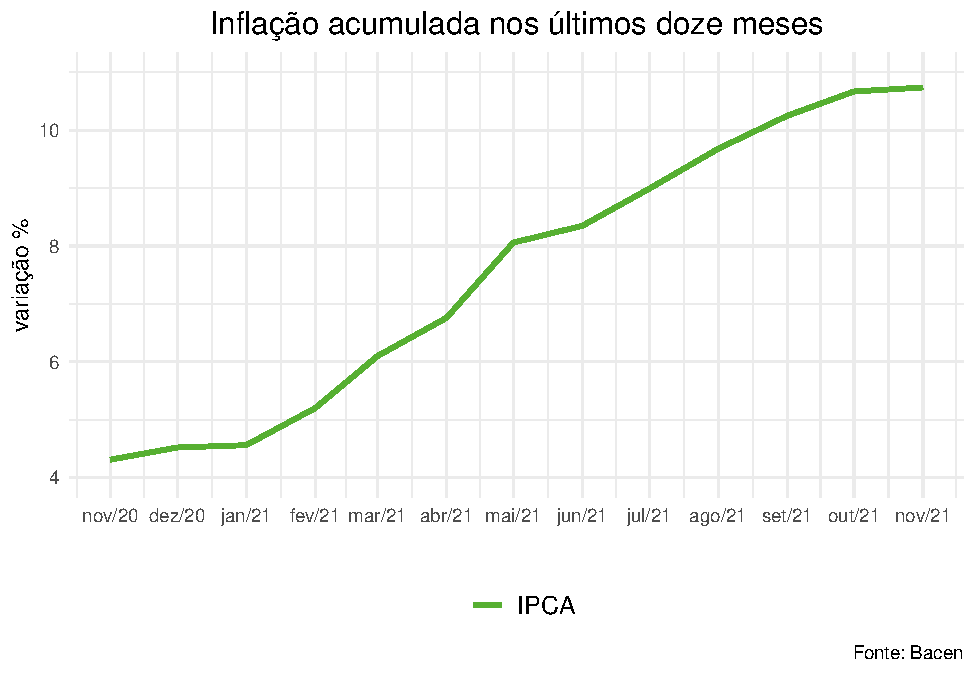
\includegraphics{inflacao_files/figure-latex/inflacao 12 meses-1.pdf}

Destaque se dá para os transportes que teve o maior aumento do índice
por três meses consecutivos, essa variação foi influenciada
principalmente pelo preço dos combustíveis, que no acumulado do ano
sofreu aumento de 50,43\%. \newpage

\section{Combustíveis} 
 \vspace{0,5cm}

A variação no preço dos combustíveis é causada por vários fatores e gera
aumento em toda cadeia de preços, visto que, a maior parte dos produtos
são dependes de transporte.

O avanço da vacinação contra a covid-19 a nível mundial proporcionou a
retomada global da economia, gerando uma grande demanda por petróleo que
não foi acompanhado da oferta, já que, no ano passado a Organização dos
Países Produtores de Petróleo (Opep) decidiu diminuir a produção para
evitar que os preços caíssem demais, com a recuperação da economia a
oferta de petróleo está sendo normalizada gradativamente, enquanto a
demanda cresce a um nível mais acelerado, provocando o aumento no preço
do barril.

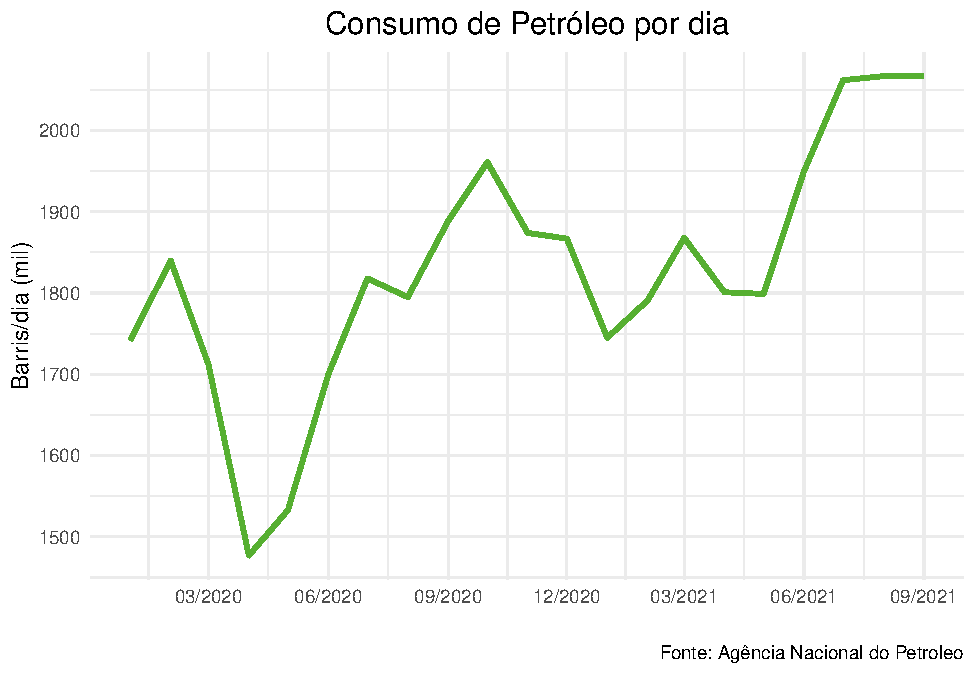
\includegraphics{inflacao_files/figure-latex/Consumo Petroleo-1.pdf}
\newpage

\section{Desvalorização Cambial} 
 \vspace{0,5cm}

O impacto desse aumento é ainda maior no Brasil devido à desvalorização
cambial, que ocorre principalmente em razão dos riscos fiscais
domésticos, a Dívida Bruta do Governo Geral (DBGG) que compreende
governo federal, INSS e governos estaduais e municipais -- atingiu
82,9\% do PIB (R\$7,0 trilhões) em outubro, essa incerteza fiscal afasta
o investimento estrangeiro.

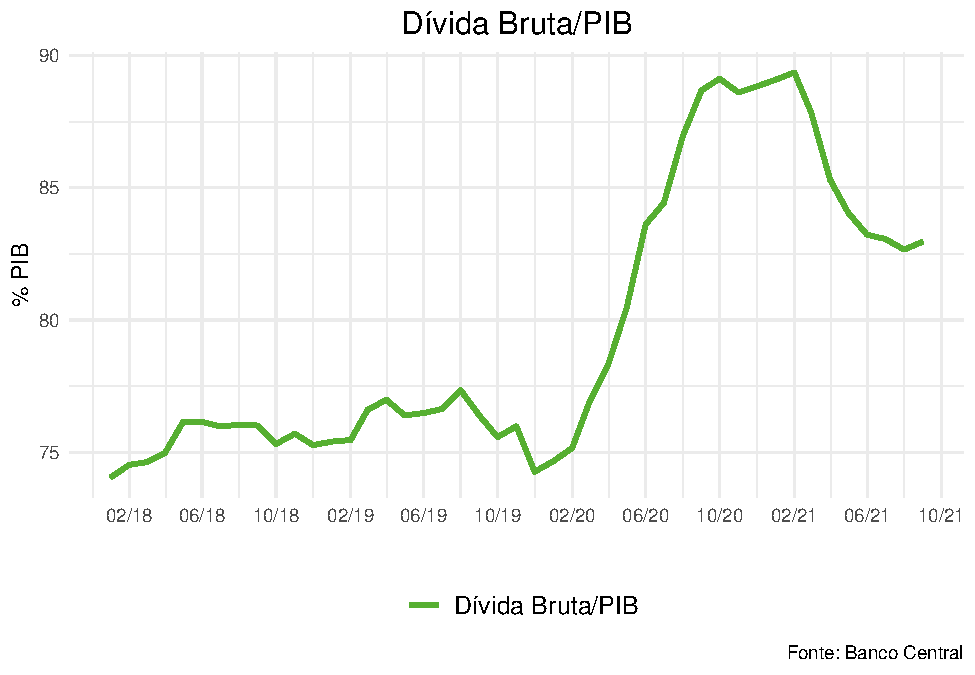
\includegraphics{inflacao_files/figure-latex/Divida Bruta/PIB-1.pdf}
\newpage

\section{Variação do Produto Interno Bruto} 
 \vspace{0,5cm}

O principal instrumento que o Comitê de Política Monetária (COPOM) tem
utilizado para controlar a inflação é o frequente aumento da taxa básica
de juros (SELIC).

No entanto, é preciso ter cautela na utilização desse mecanismo, visto
que, ele impacta também no Produto Interno Bruto (PIB), que teve
variação negativa por dois trimestres consecutivos, fazendo com que o
Brasil entrasse em resseção técnica

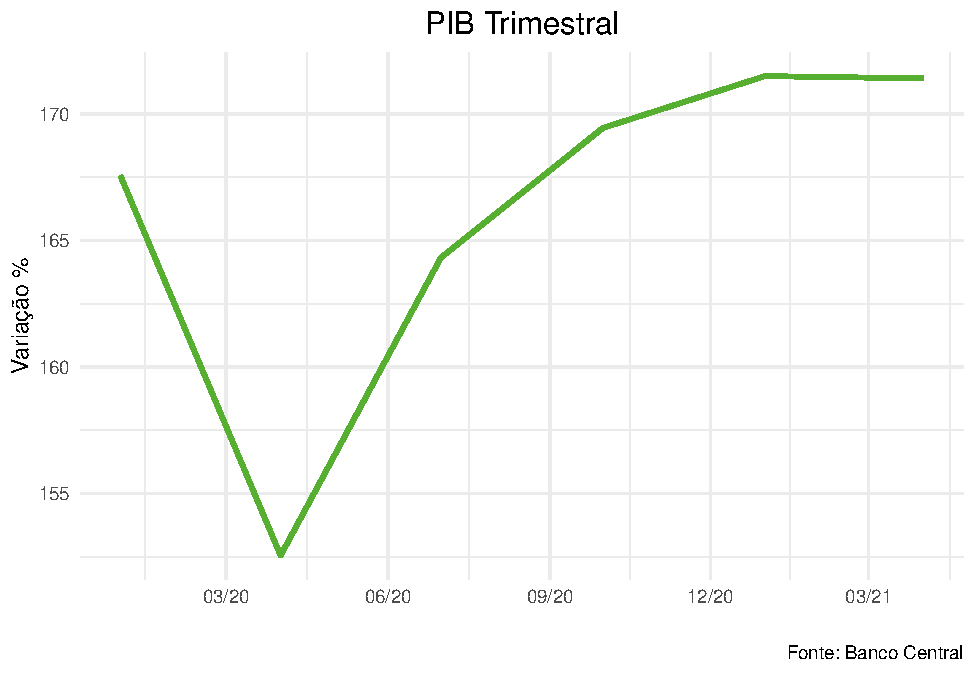
\includegraphics{inflacao_files/figure-latex/PIB trimestral-1.pdf}

O aumento da Selic, impacta diretamente o custo do crédito,
desacelerando o investimento. Além disso, segundo o próprio Banco
Central, o impacto da taxa SELIC na inflação leva em média entre 6 a 9
meses para ocorrer.

\newpage

\section{Inflação - Grande Vitória} 
 \vspace{0,25cm}

A Grande Vitória ocupa o segundo lugar no ranking das capitais com maior
índice de inflação, com alta de 9,58\% no acumulado do ano, ficando
atrás apenas de Curitiba que teve variação de 10,97\%. Em relação a
variação mensal a capital atingiu 1,53\%, ocupando o primeiro lugar do
ranking.

Destaque para a habitação que no acumulado do ano obteve a segunda maior
alta do Brasil, com variação de 15,01\%, durante o mês de outubro foi o
item com maior alta da Grande Vitória, o aumento de 3,04\% foi
impulsionado principalmente pelo subitem gás de botija, que teve alta de
5,41\% em relação ao mês anterior.

No que se refere aos alimentos e bebidas foi a maior alta do país, com
aumento de 2,48\% em relação ao mês anterior, e variação de 7,43\% no
acumulado do ano. De acordo com o Dieese, o valor da cesta básica em
setembro na Grande Vitória foi de R\$633,03.

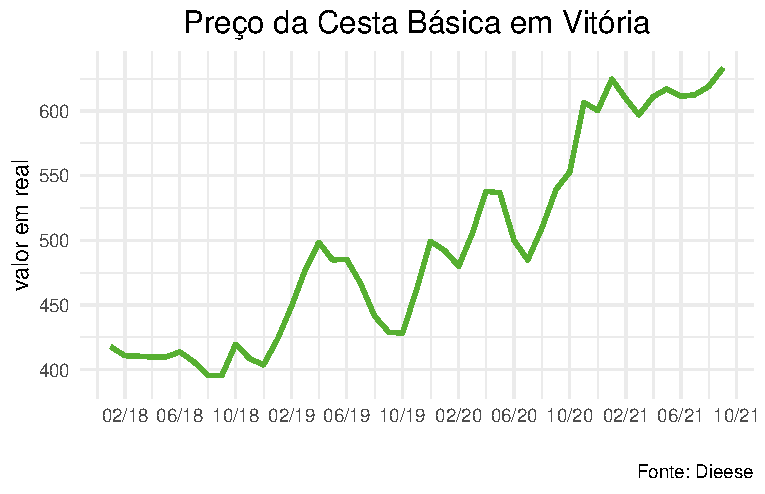
\includegraphics{inflacao_files/figure-latex/IPCA es-1.pdf}


\end{document}
